%@ chapter=5
%@ exercise=1
%@ author=Fabian

Let $\tuple{a}{b}$ be a pullback of $f$ and $g$, then the following diagram in $\cat{C}$ commutes.

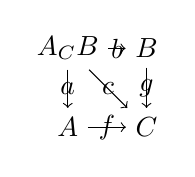
\begin{tikzpicture}
  \node (AxCB) {$A ×_C B$};
  \node (A) [below of=AxCB] {$A$};
  \node (B) [right of=AxCB] {$B$};
  \node (C) [right of=A] {$C$};
  \draw[->] (A) to node {$f$} (C);
  \draw[->] (B) to node {$g$} (C);
  \draw[->] (AxCB) to node {$a$} (A);
  \draw[->] (AxCB) to node {$b$} (B);
  \draw[->] (AxCB) to node {$c$} (C);
\end{tikzpicture}

Here, $c = f ∘ a = g ∘ b$ is the composition of the pullback edges. Constructing the slice category $\qcat{C}{C}$, we obtain the following diagram.

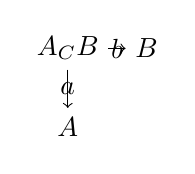
\begin{tikzpicture}
  \node (AxCB) {$A ×_C B$};
  \node (A) [below of=AxCB] {$A$};
  \node (B) [right of=AxCB] {$B$};
  \draw[->] (AxCB) to node {$a$} (A);
  \draw[->] (AxCB) to node {$b$} (B);
\end{tikzpicture}

Now, we prove that object $A ×_C B \in \qcat{C}{C}$ fulfills the universal property of a product of $A$ and $B$. Therefore, assume some object $X$ with arrows to $A$ and $B$. Since $\qcat{C}{C}$ is the slice category of $C$ in $\cat{C}$, there exists an arrow $h : X → C$ in $\cat{C}$ and arrows $a' : X → A$, $b' : X → B$ so that $h = f ∘ a' = g ∘ b'$. Hence, the following diagram in $\cat{C}$ commutes.

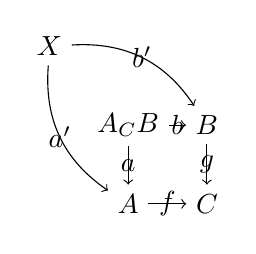
\begin{tikzpicture}
  \node (AxCB) {$A ×_C B$};
  \node (X) [left of=AxCB, above of=AxCB] {$X$};
  \node (A) [below of=AxCB] {$A$};
  \node (B) [right of=AxCB] {$B$};
  \node (C) [right of=A] {$C$};
  \draw[->] (A) to node {$f$} (C);
  \draw[->] (B) to node {$g$} (C);
  \draw[->] (AxCB) to node {$a$} (A);
  \draw[->] (AxCB) to node {$b$} (B);
  \draw[->, bend right] (X) to node {$a'$} (A);
  \draw[->, bend left] (X) to node {$b'$} (B);
\end{tikzpicture}

From the universal property of $A ×_C B$ as pullback we obtain the existence of a unique arrow $u : X → A ×_C B$ so that $a' = a ∘ u$ and $b' = b ∘ u$. Thus, $u$ is a morphism from $X$ to $A ×_C B$ in the slice category $\qcat{C}{C}$. To conclude the proof, we observe that any morphism $• : X → A ×_C B$ that lets the diagram in $\qcat{C}{C}$ commute, lets the diagram in $\cat{C}$ commute when substituted for $u$. Therefore, both $u$ is unique in $\qcat{C}{C}$ and given the product of $A$ and $B$ in $\qcat{C}{C}$, that is the same as the pullback of $A$ and $B$ in $\cat{C}$.
